\chapter{Additional Graphics}
\label{app:addional_graphics}


\begin{figure}[htb!]
    \centering
    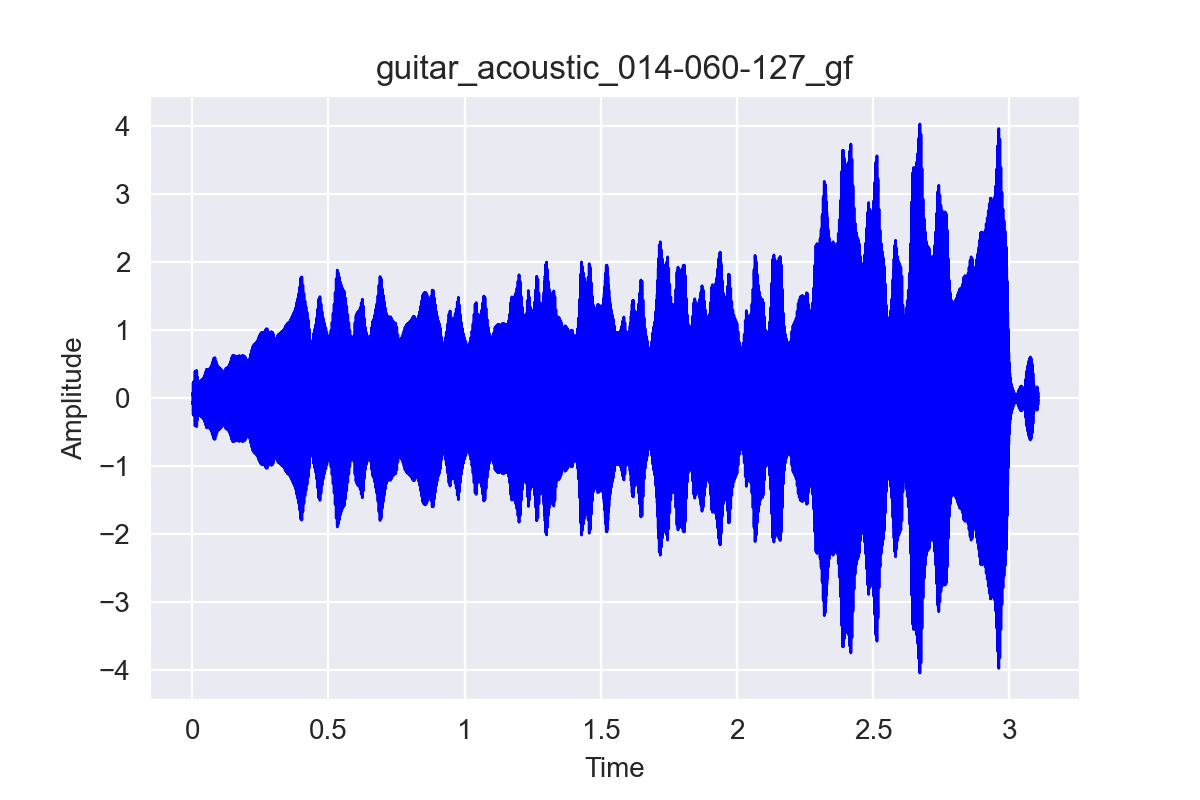
\includegraphics[width=0.60\textwidth]{images/appendix/1D/guitar_acoustic_014-060-127_gf.png}
    \caption{Acoustic guitar output with Griffin-Lim (1D conv).}
    
\end{figure}


\begin{figure}[htb!]
    \centering
    \captionsetup{justification=centering}
    \makebox[\textwidth][c]{\begin{tabular}{@{}cc@{}}
        \makebox{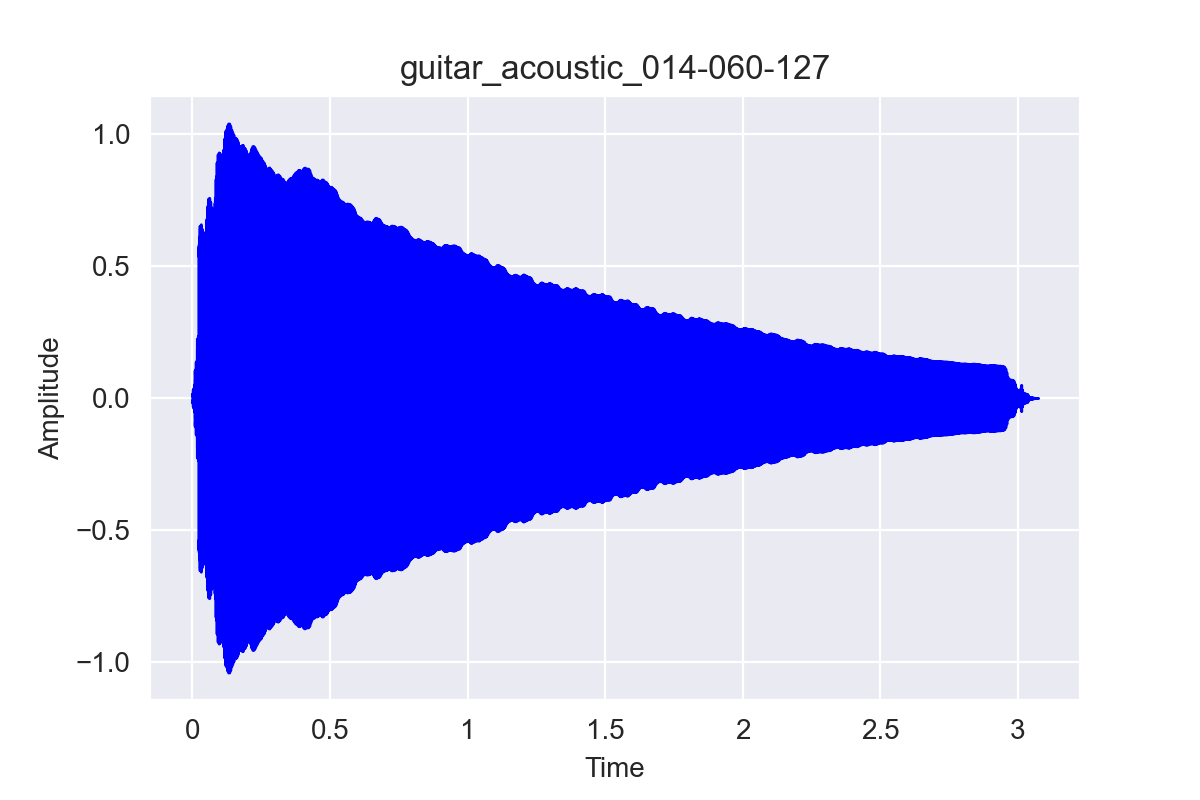
\includegraphics[width=0.5\textwidth]{images/appendix/single_stride/guitar_acoustic_014-060-127.png}}&
        \makebox{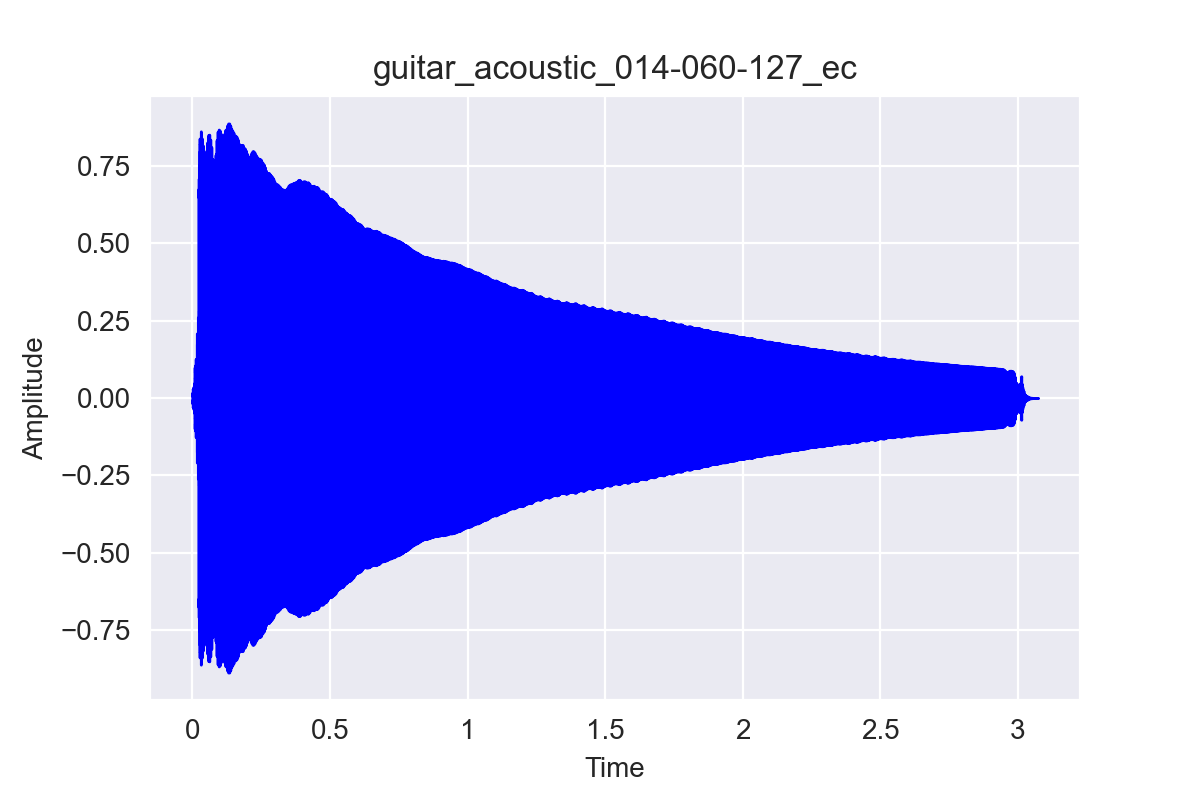
\includegraphics[width=0.5\textwidth]{images/appendix/single_stride/guitar_acoustic_014-060-127_ec.png}}\\
        without post-processing ~(a) & with post-processing ~(b)
    \end{tabular}}
    \caption{Difference between acoustic guitar output signals without and with post-processing using 2D convolutional single-stride network and original phase.}
    
\end{figure}

\begin{figure}[htb!]
    \centering
    \captionsetup{justification=centering}
    \makebox[\textwidth][c]{\begin{tabular}{@{}cc@{}}
        \makebox{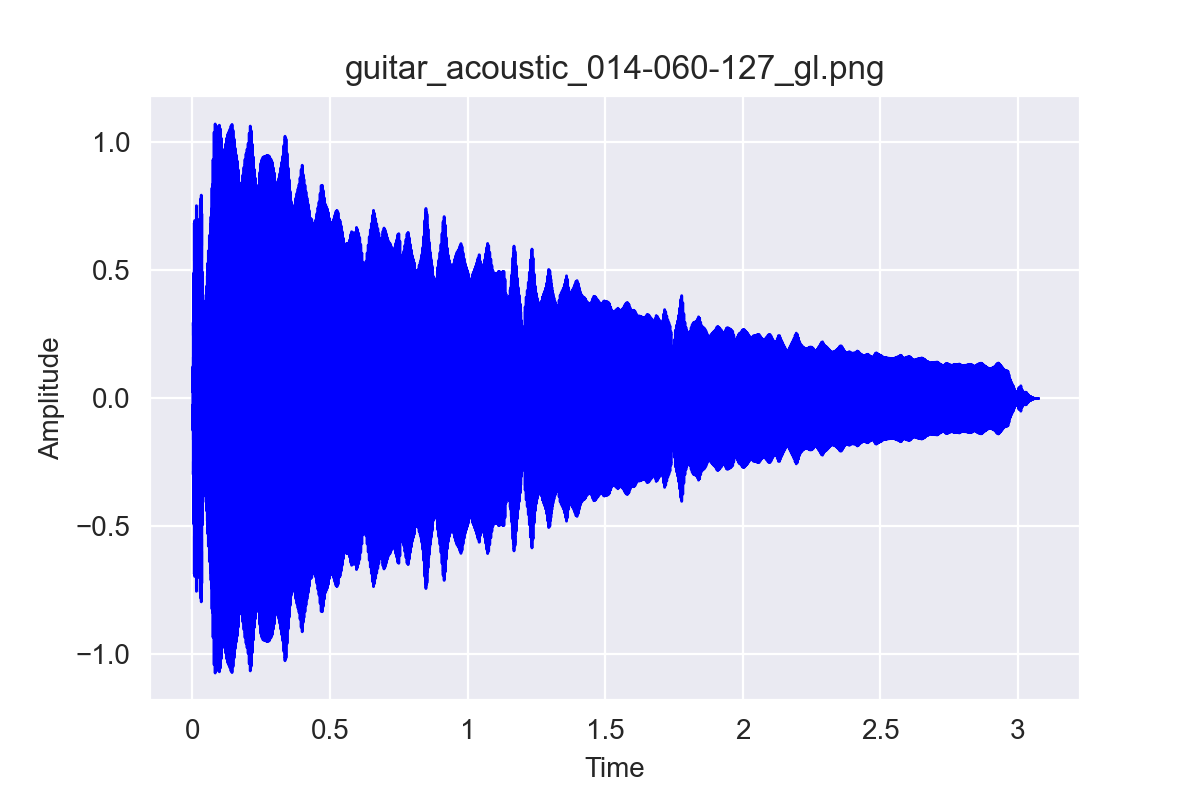
\includegraphics[width=0.5\textwidth]{images/appendix/single_stride/guitar_acoustic_014-060-127_gl.png}}&
        \makebox{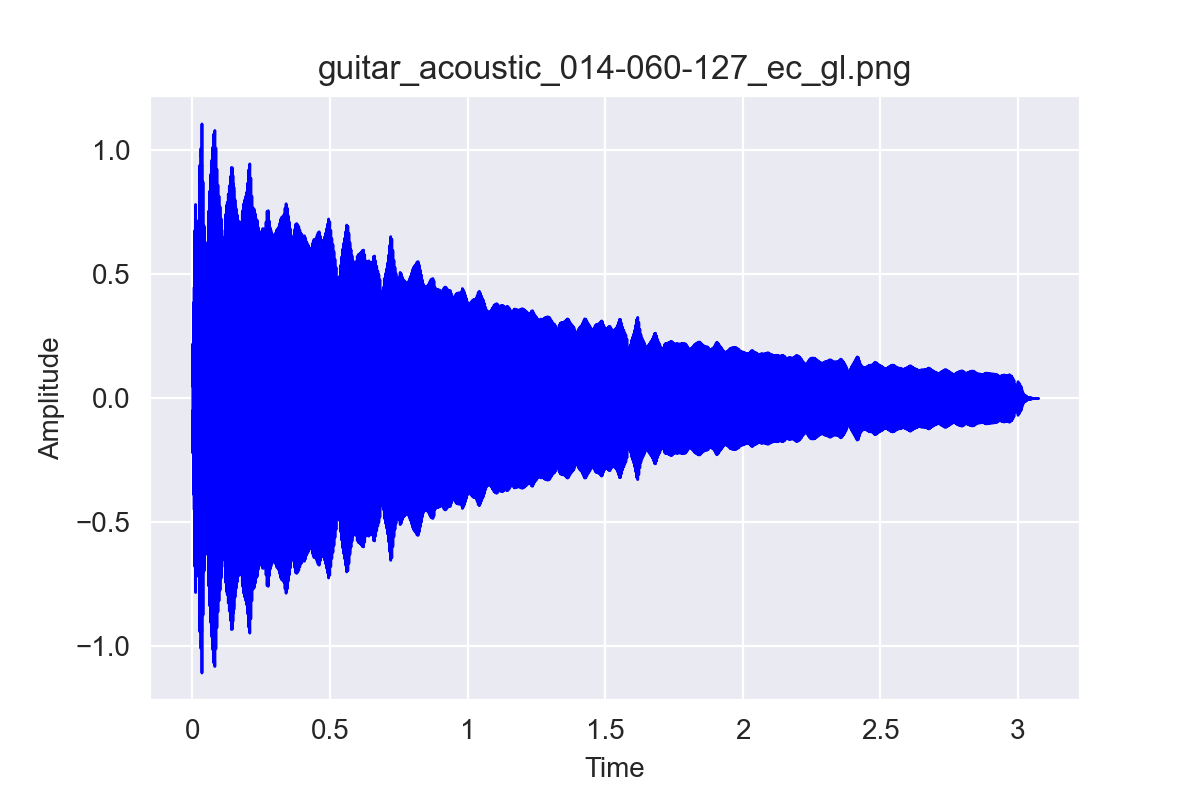
\includegraphics[width=0.5\textwidth]{images/appendix/single_stride/guitar_acoustic_014-060-127_ec_gl.png}}\\
        without post-processing ~(a) & with post-processing ~(b)
    \end{tabular}}
    \caption{Difference between acoustic guitar output signals without and with post-processing using 2D convolutional single-stride network and Griffin-Lim.}
    
\end{figure}

\begin{figure}[htb!]
    \centering
    \captionsetup{justification=centering}
    \makebox[\textwidth][c]{\begin{tabular}{@{}cc@{}}
        \makebox{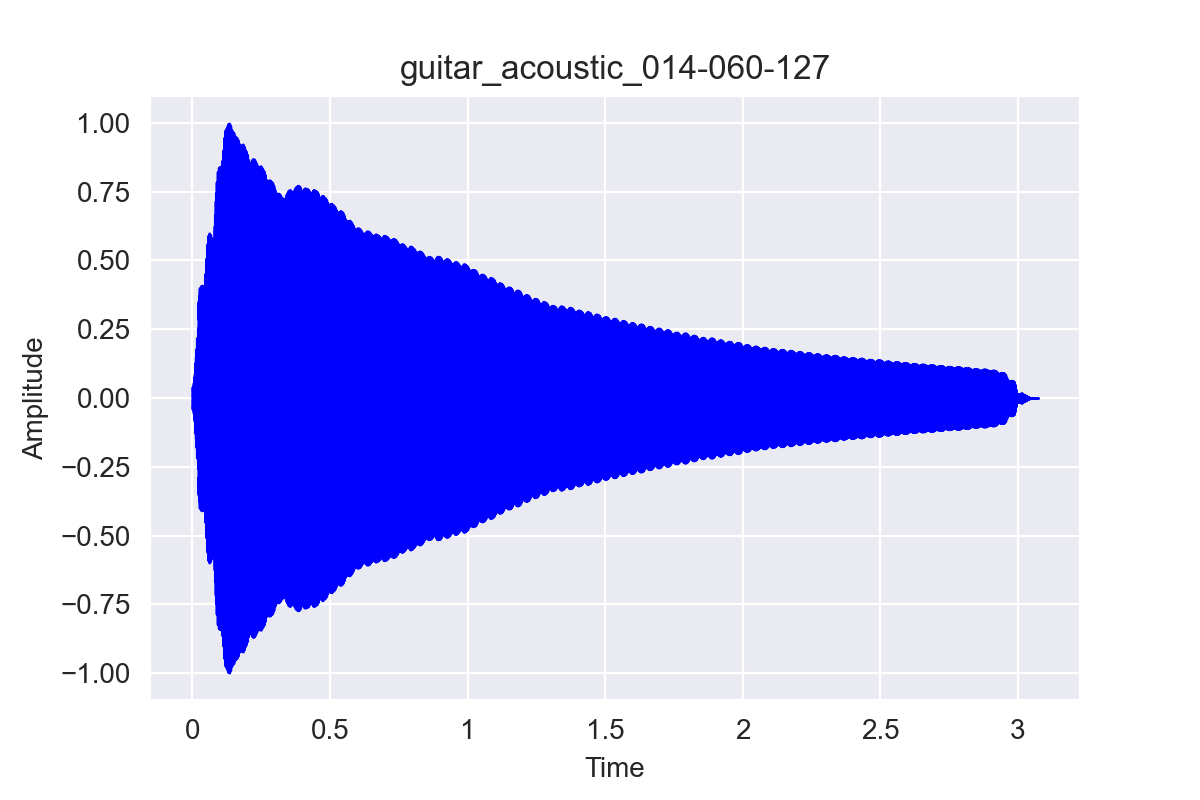
\includegraphics[width=0.5\textwidth]{images/appendix/double_stride/guitar_acoustic_014-060-127.png}}&
        \makebox{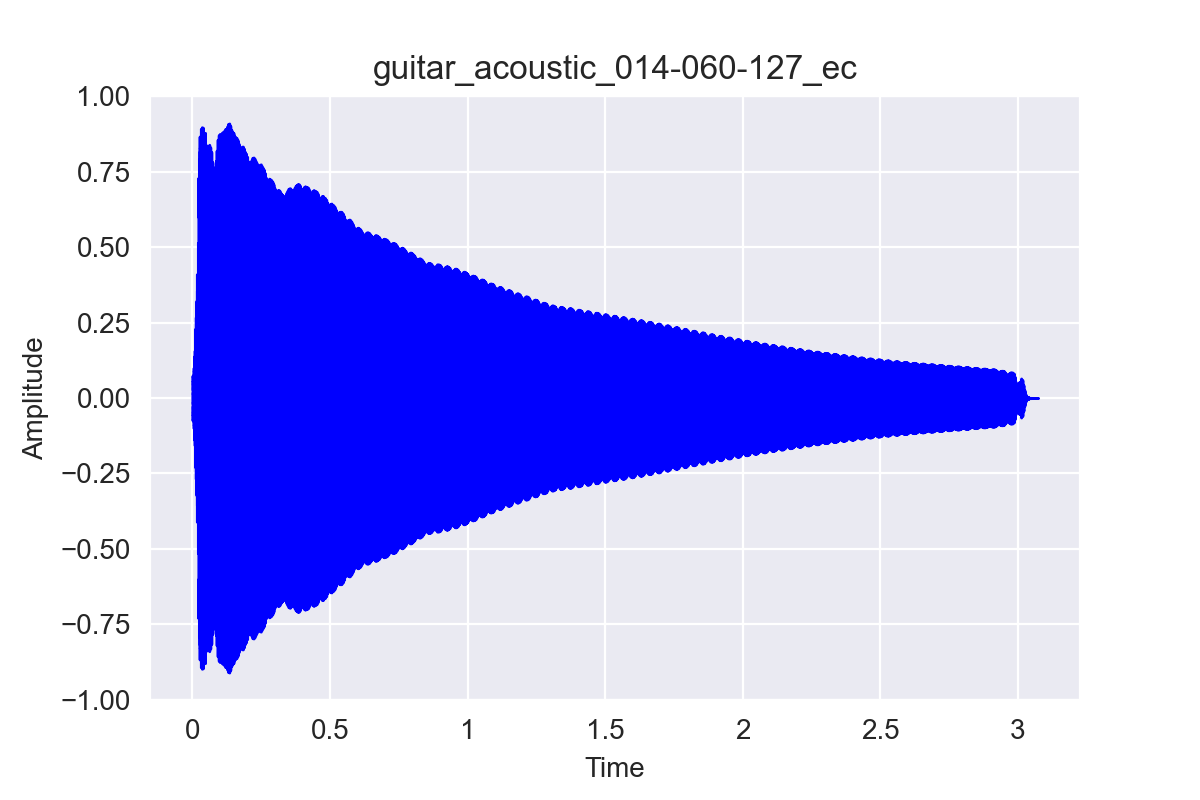
\includegraphics[width=0.5\textwidth]{images/appendix/double_stride/guitar_acoustic_014-060-127_ec.png}}\\
        without post-processing ~(a) & with post-processing ~(b)
    \end{tabular}}
    \caption{Difference between acoustic guitar output signals without and with post-processing using 2D convolutional double-stride network and original phase.}
    
\end{figure}

\begin{figure}[htb!]
    \centering
    \captionsetup{justification=centering}
    \makebox[\textwidth][c]{\begin{tabular}{@{}cc@{}}
        \makebox{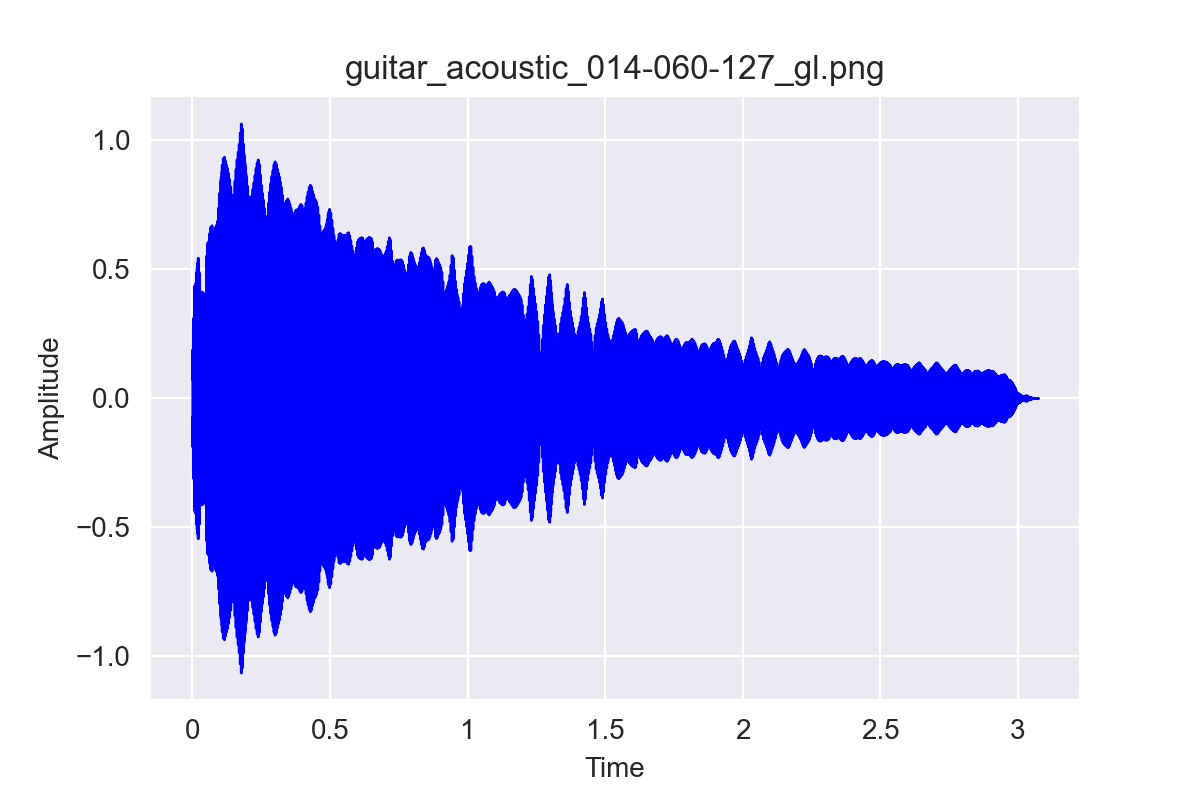
\includegraphics[width=0.50\textwidth]{images/appendix/double_stride/guitar_acoustic_014-060-127_gl.png}}&
        \makebox{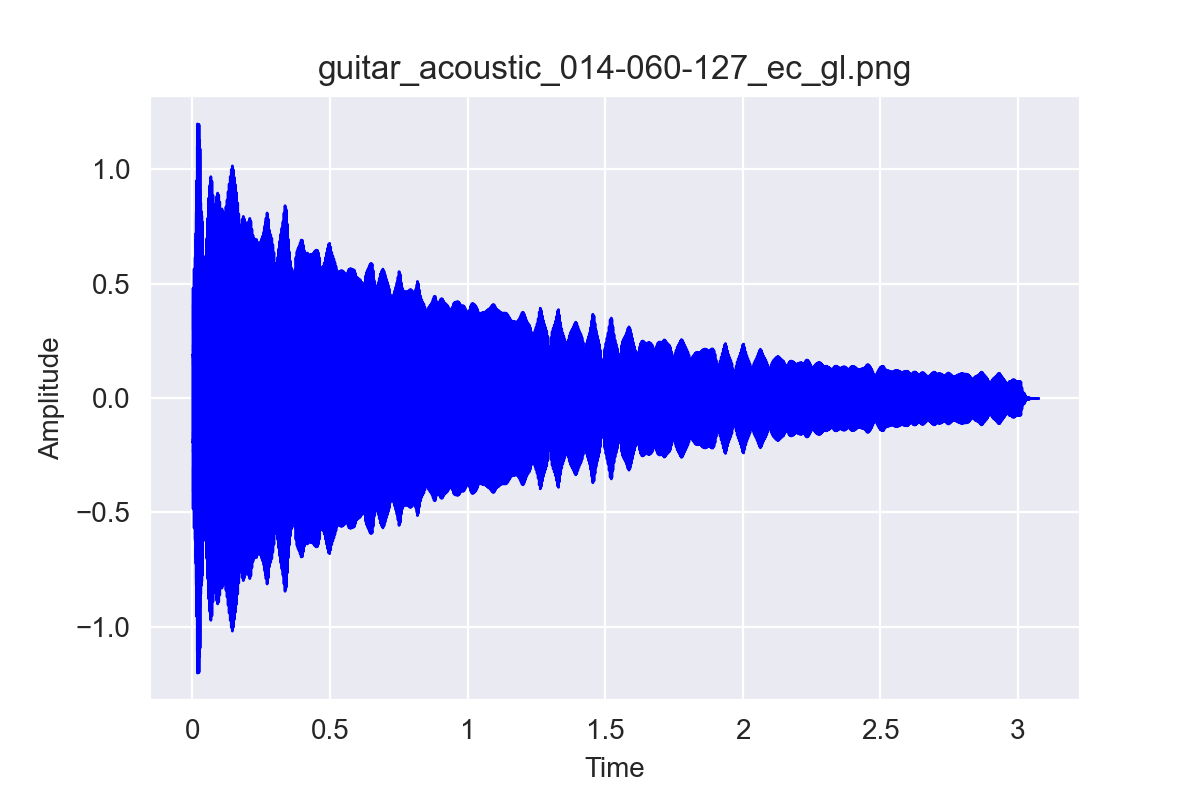
\includegraphics[width=0.50\textwidth]{images/appendix/double_stride/guitar_acoustic_014-060-127_ec_gl.png}}\\
        without post-processing ~(a) & with post-processing ~(b)
    \end{tabular}}
    \caption{Difference between acoustic guitar output signals without and with post-processing using 2D convolutional double-stride network and Griffin-Lim.}
    
\end{figure}

\begin{figure}[htb!]
    \centering
    \captionsetup{justification=centering}
    \makebox[\textwidth][c]{\begin{tabular}{@{}cc@{}}
        \makebox{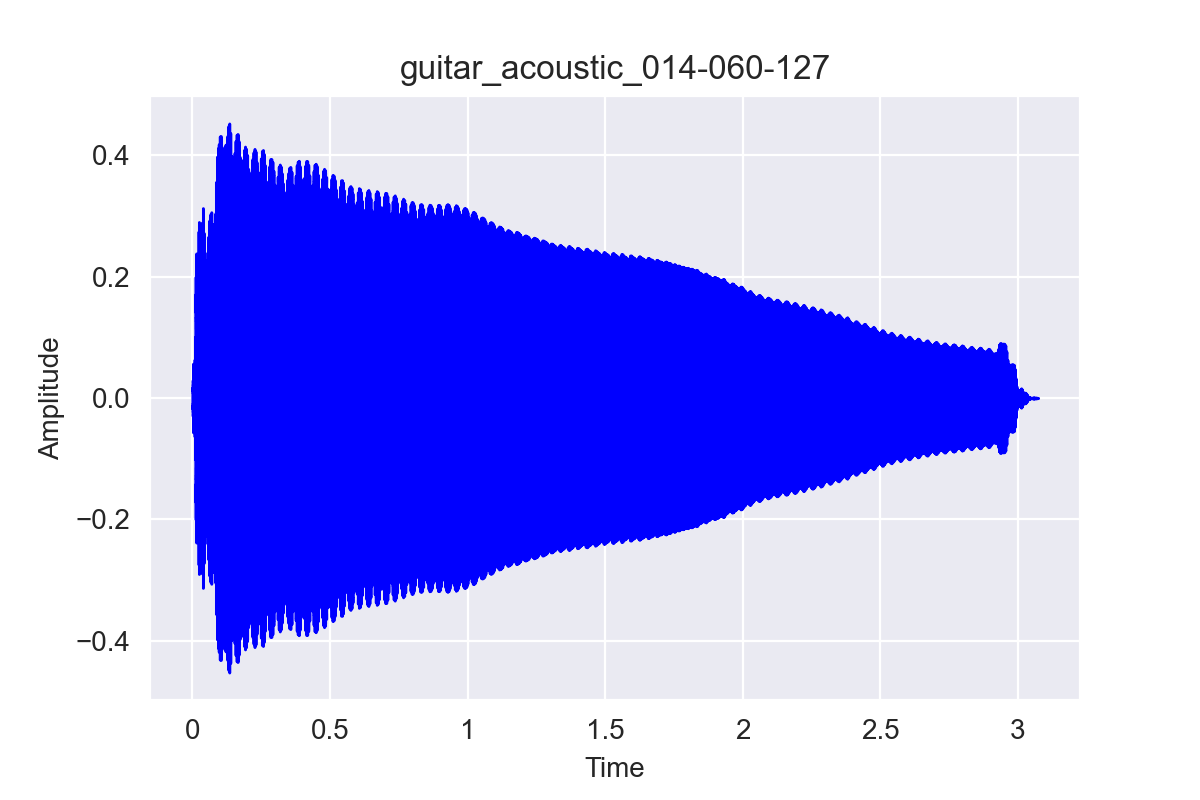
\includegraphics[width=0.50\textwidth]{images/appendix/triple_stride/guitar_acoustic_014-060-127.png}}&
        \makebox{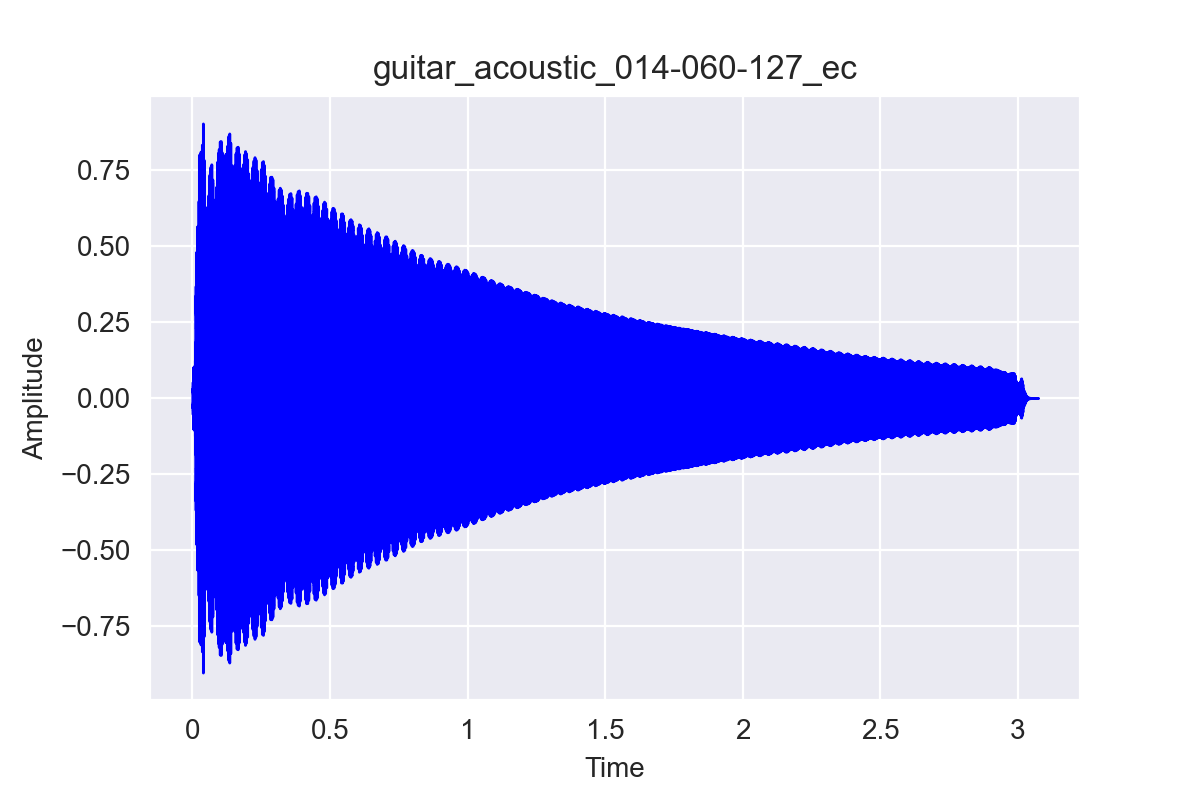
\includegraphics[width=0.50\textwidth]{images/appendix/triple_stride/guitar_acoustic_014-060-127_ec.png}}\\
        without post-processing ~(a) & with post-processing ~(b)
    \end{tabular}}
    \caption{Difference between acoustic guitar output signals without and with post-processing using 2D convolutional triple-stride network and original phase.}
    
\end{figure}

\begin{figure}[htb!]
    \centering
    \captionsetup{justification=centering}
    \makebox[\textwidth][c]{\begin{tabular}{@{}cc@{}}
        \makebox{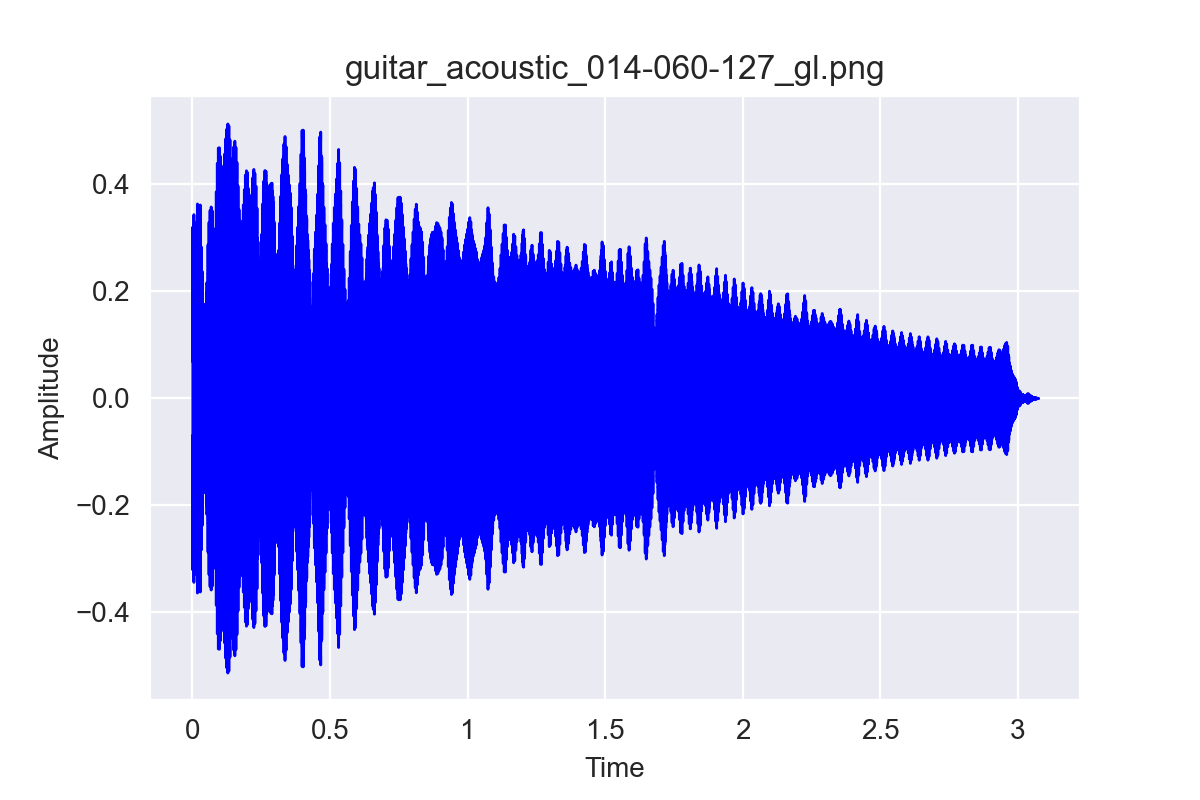
\includegraphics[width=0.50\textwidth]{images/appendix/triple_stride/guitar_acoustic_014-060-127_gl.png}}&
        \makebox{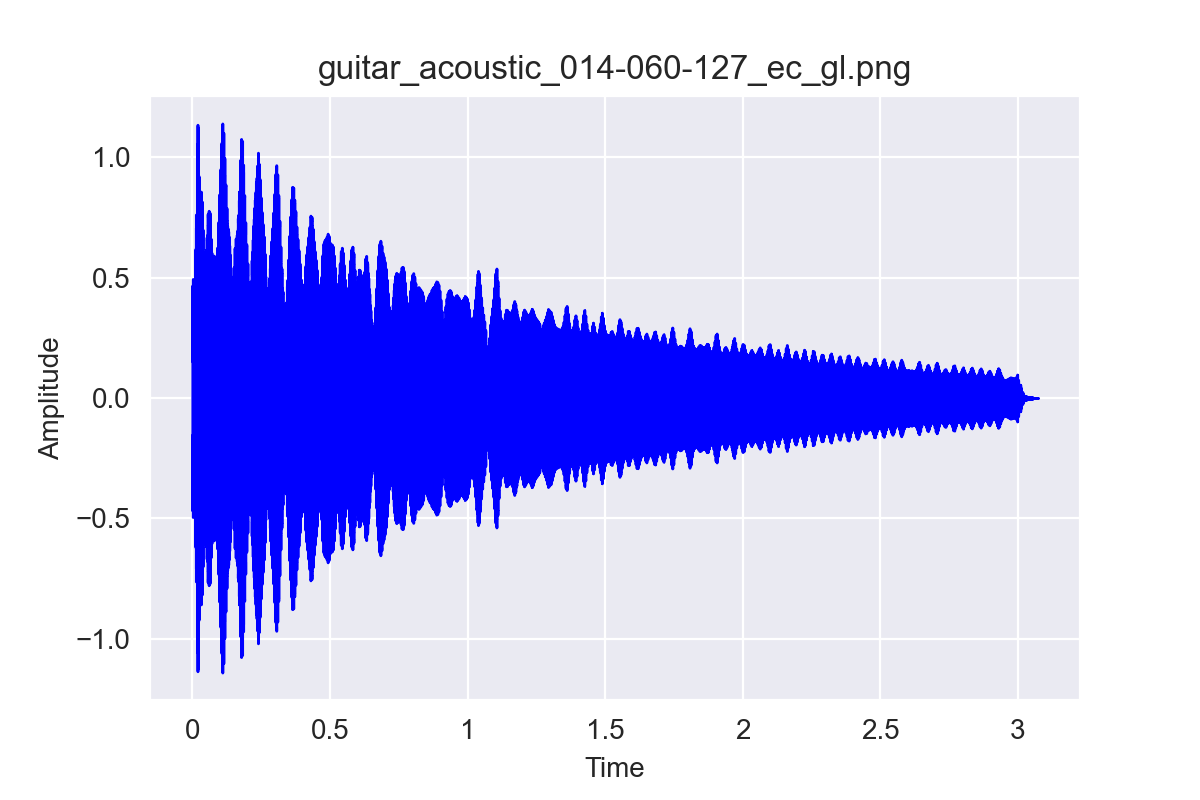
\includegraphics[width=0.50\textwidth]{images/appendix/triple_stride/guitar_acoustic_014-060-127_ec_gl.png}}\\
        without post-processing ~(a) & with post-processing ~(b)
    \end{tabular}}
    \caption{Difference between acoustic guitar output signals without and with post-processing using 2D convolutional triple-stride network and Griffin-Lim.}
    
\end{figure}


\begin{figure}[htb!]
    \centering
    \captionsetup{justification=centering}
    \makebox[\textwidth][c]{\begin{tabular}{@{}cc@{}}
        \makebox{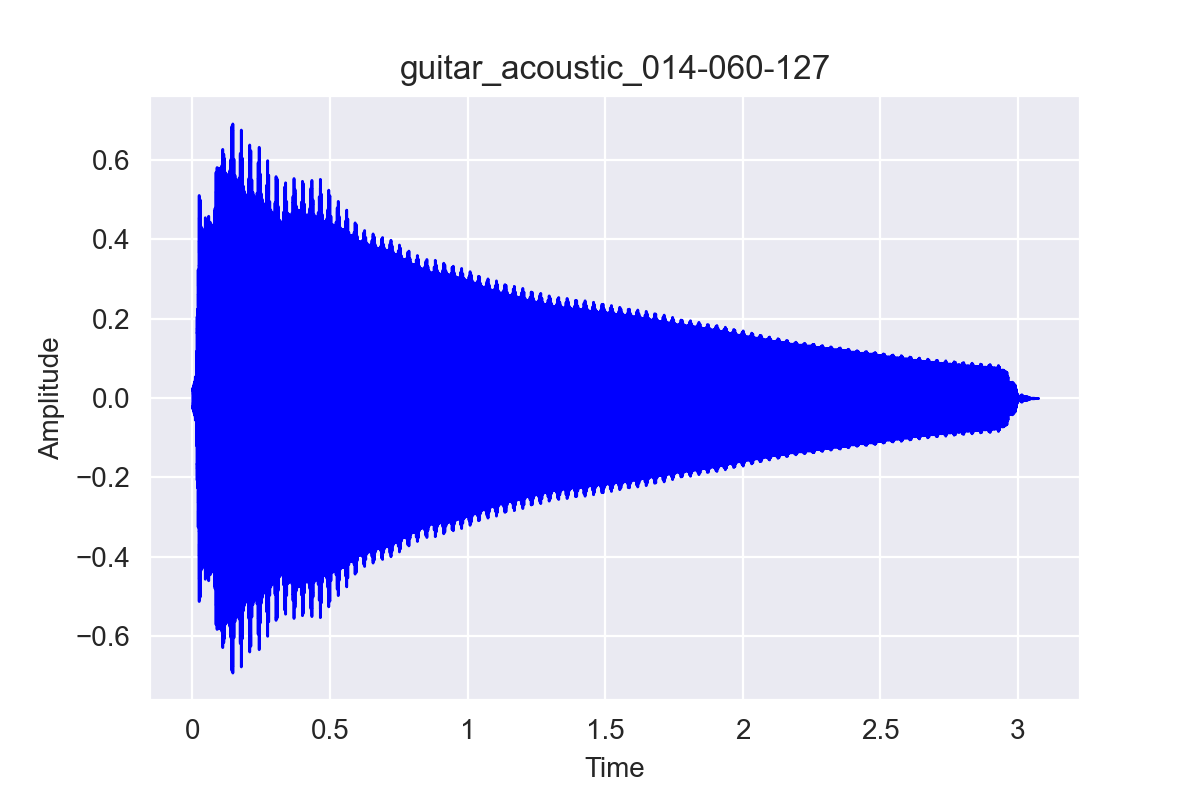
\includegraphics[width=0.50\textwidth]{images/appendix/mel_single_stride/guitar_acoustic_014-060-127.png}}&
        \makebox{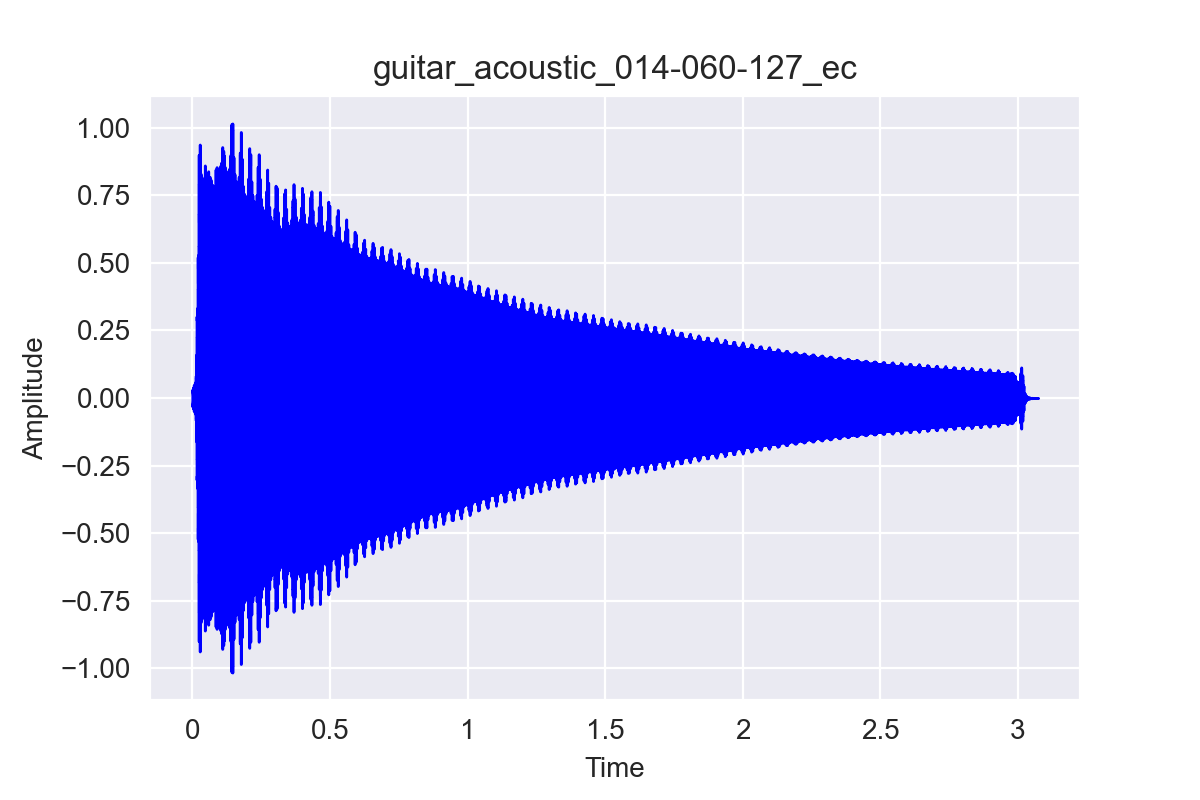
\includegraphics[width=0.50\textwidth]{images/appendix/mel_single_stride/guitar_acoustic_014-060-127_ec.png}}\\
        without post-processing ~(a) & with post-processing ~(b)
    \end{tabular}}
    \caption{Difference between acoustic guitar output signals without and with post-processing using 2D convolutional single-stride network and original phase with log-mel spectrograms.}
    
\end{figure}

\begin{figure}[htb!]
    \centering
    \captionsetup{justification=centering}
    \makebox[\textwidth][c]{\begin{tabular}{@{}cc@{}}
        \makebox{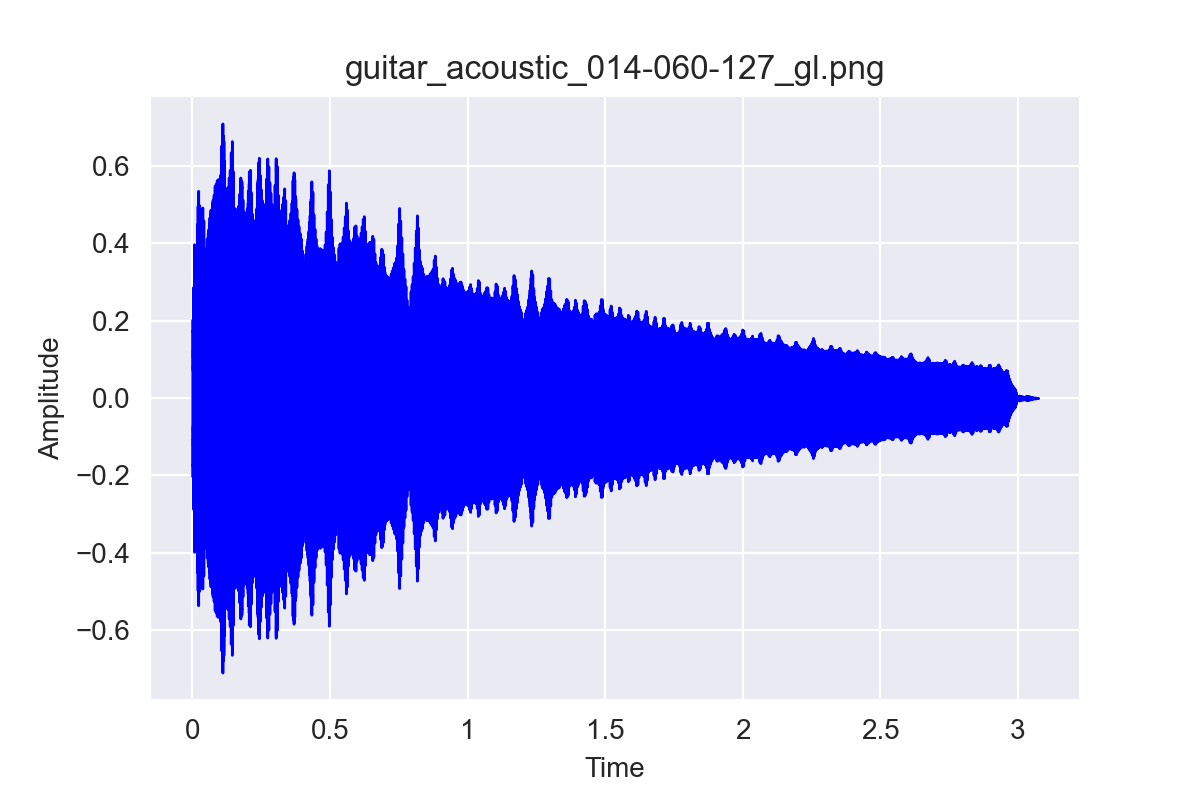
\includegraphics[width=0.50\textwidth]{images/appendix/mel_single_stride/guitar_acoustic_014-060-127_gl.png}}&
        \makebox{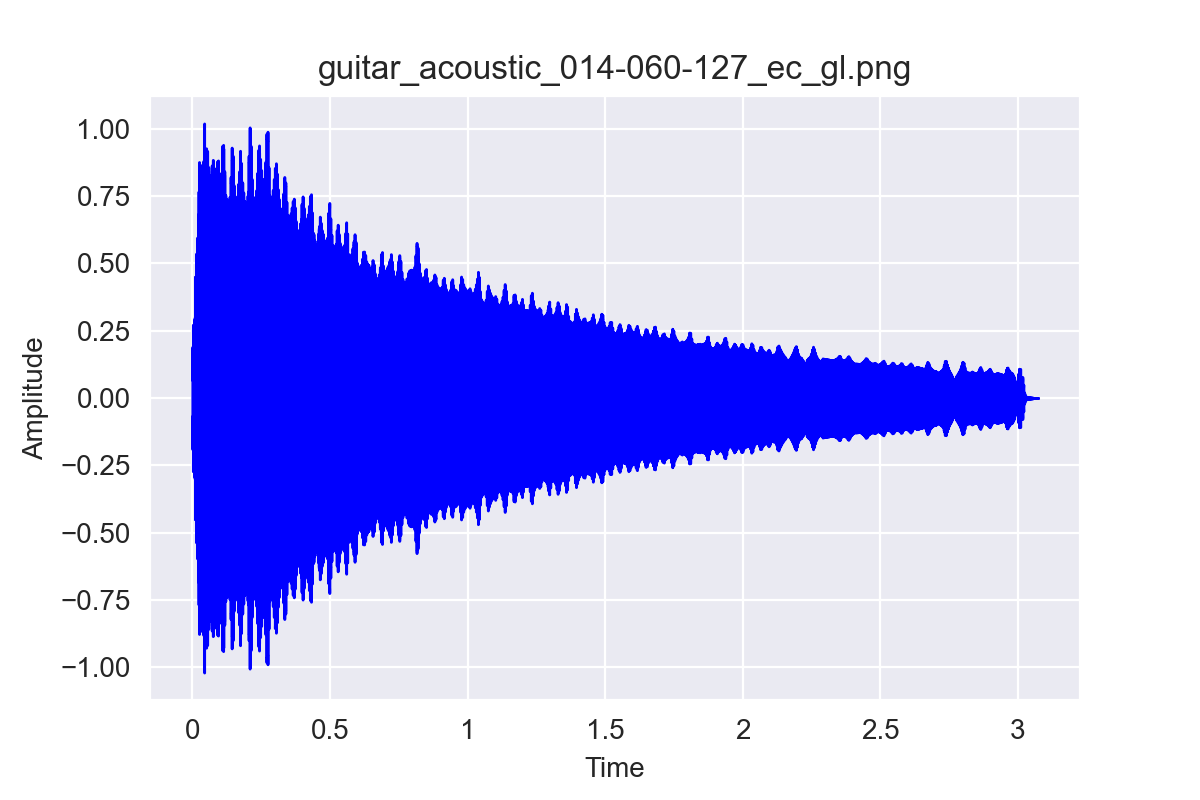
\includegraphics[width=0.50\textwidth]{images/appendix/mel_single_stride/guitar_acoustic_014-060-127_ec_gl.png}}\\
        without post-processing ~(a) & with post-processing ~(b)
    \end{tabular}}
    \caption{Difference between acoustic guitar output signals without and with post-processing using 2D convolutional single-stride network and Griffin-Lim with log-mel spectrograms.}
    
\end{figure}

\begin{figure}[htb!]
    \centering
    \captionsetup{justification=centering}
    \makebox[\textwidth][c]{\begin{tabular}{@{}cc@{}}
        \makebox{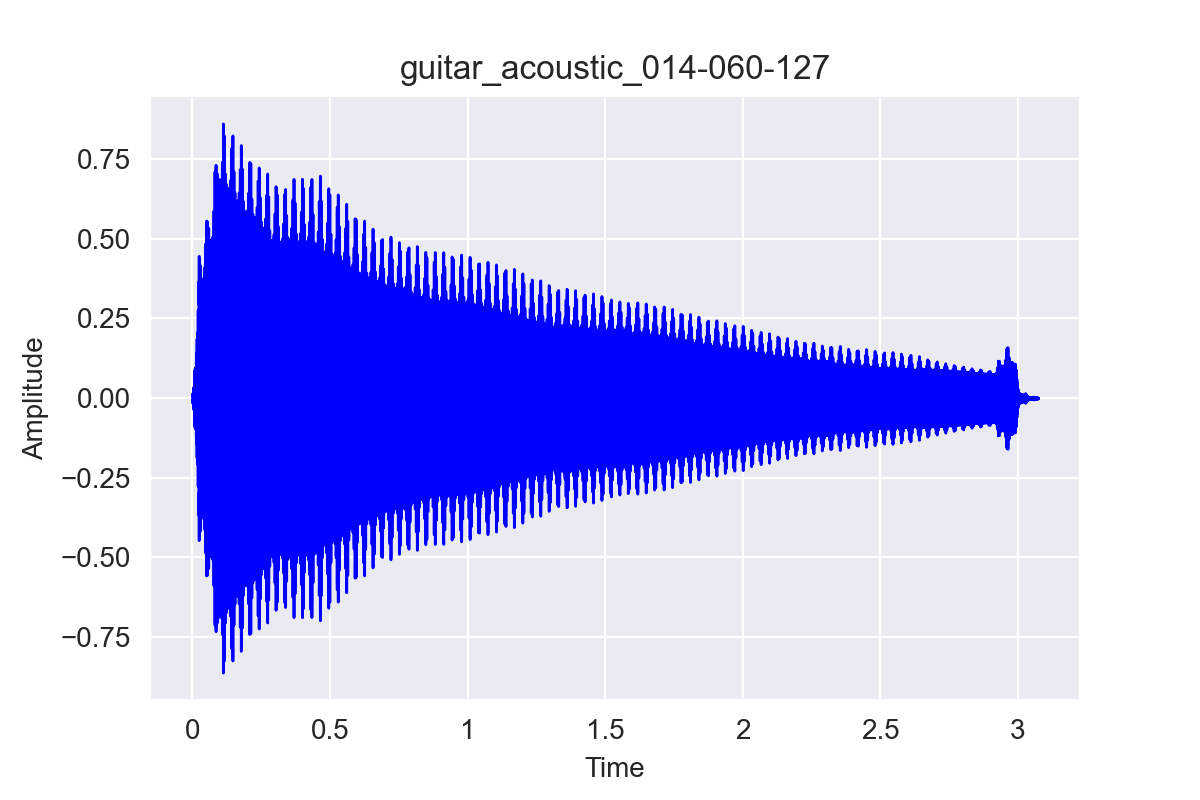
\includegraphics[width=0.50\textwidth]{images/appendix/mel_double_stride/guitar_acoustic_014-060-127.png}}&
        \makebox{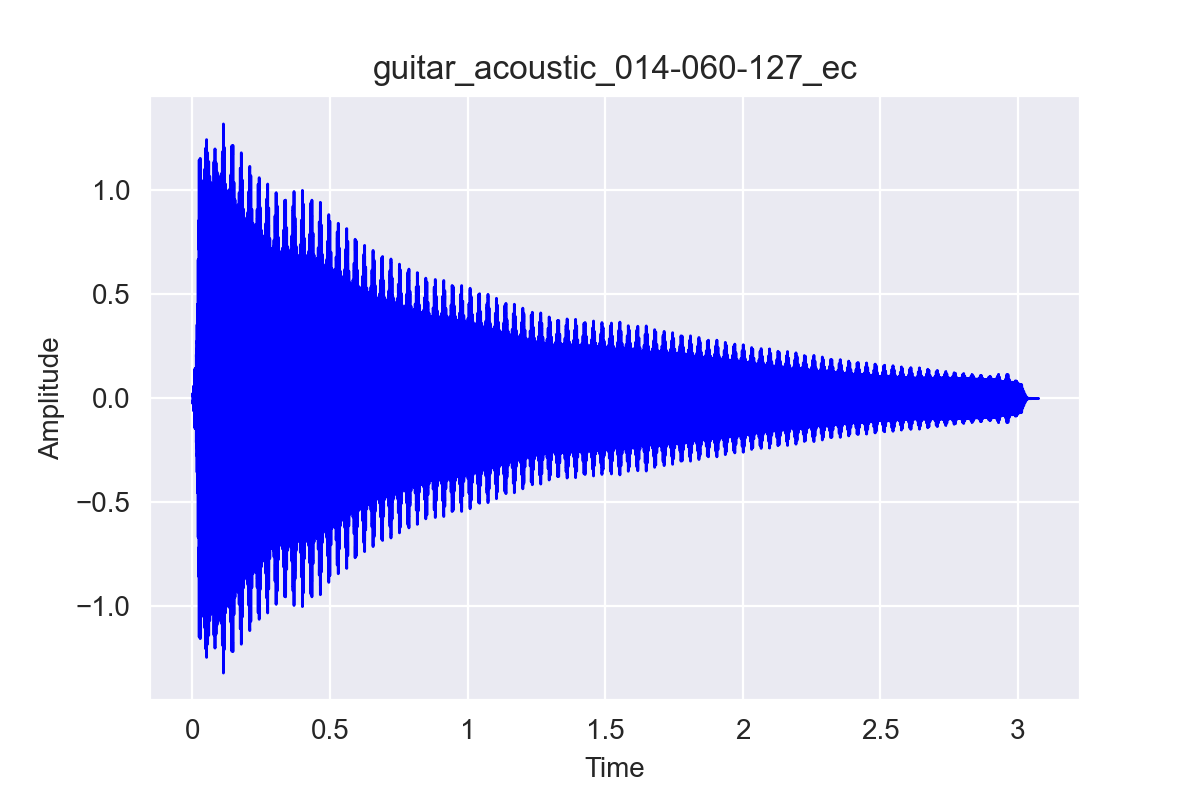
\includegraphics[width=0.50\textwidth]{images/appendix/mel_double_stride/guitar_acoustic_014-060-127_ec.png}}\\
        without post-processing ~(a) & output with post-processing ~(b)
    \end{tabular}}
    \caption{Difference between acoustic guitar output signals without and with post-processing using 2D convolutional double-stride network and original phase with log-mel spectrograms.}
    
\end{figure}

\begin{figure}[htb!]
    \centering
    \captionsetup{justification=centering}
    \makebox[\textwidth][c]{\begin{tabular}{@{}cc@{}}
        \makebox{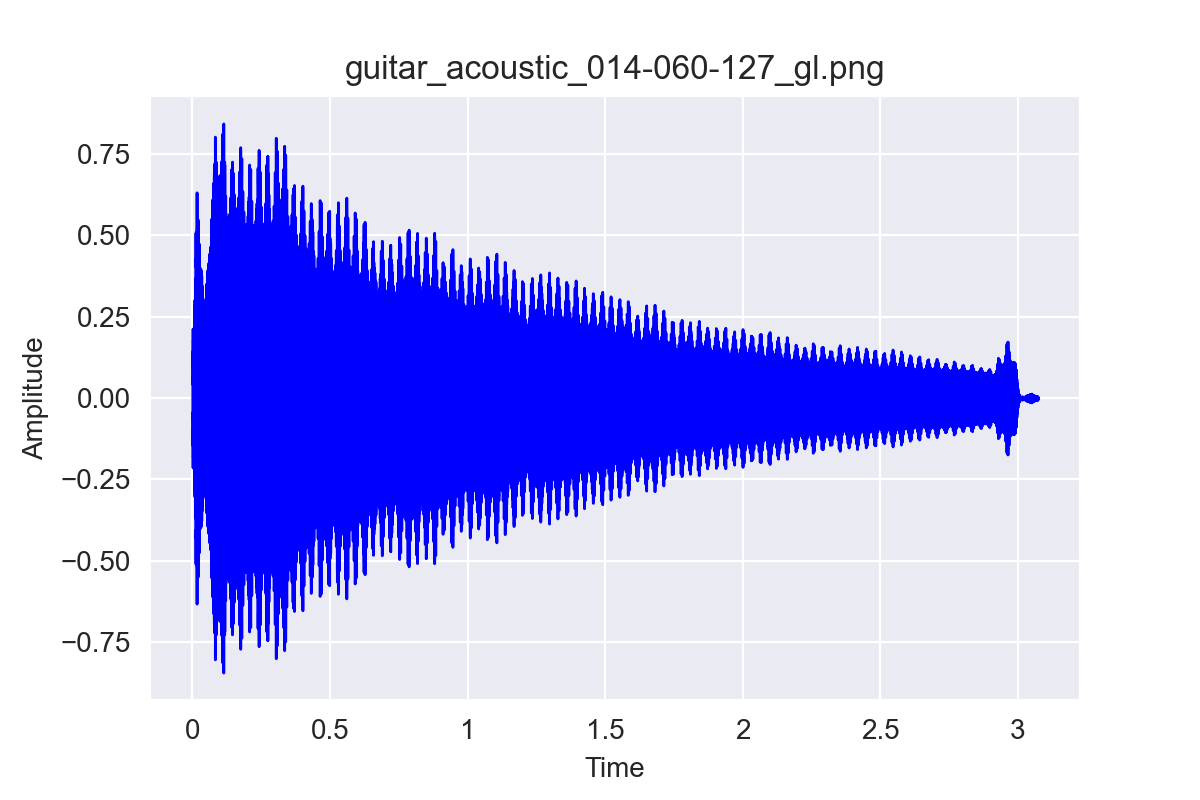
\includegraphics[width=0.50\textwidth]{images/appendix/mel_double_stride/guitar_acoustic_014-060-127_gl.png}}&
        \makebox{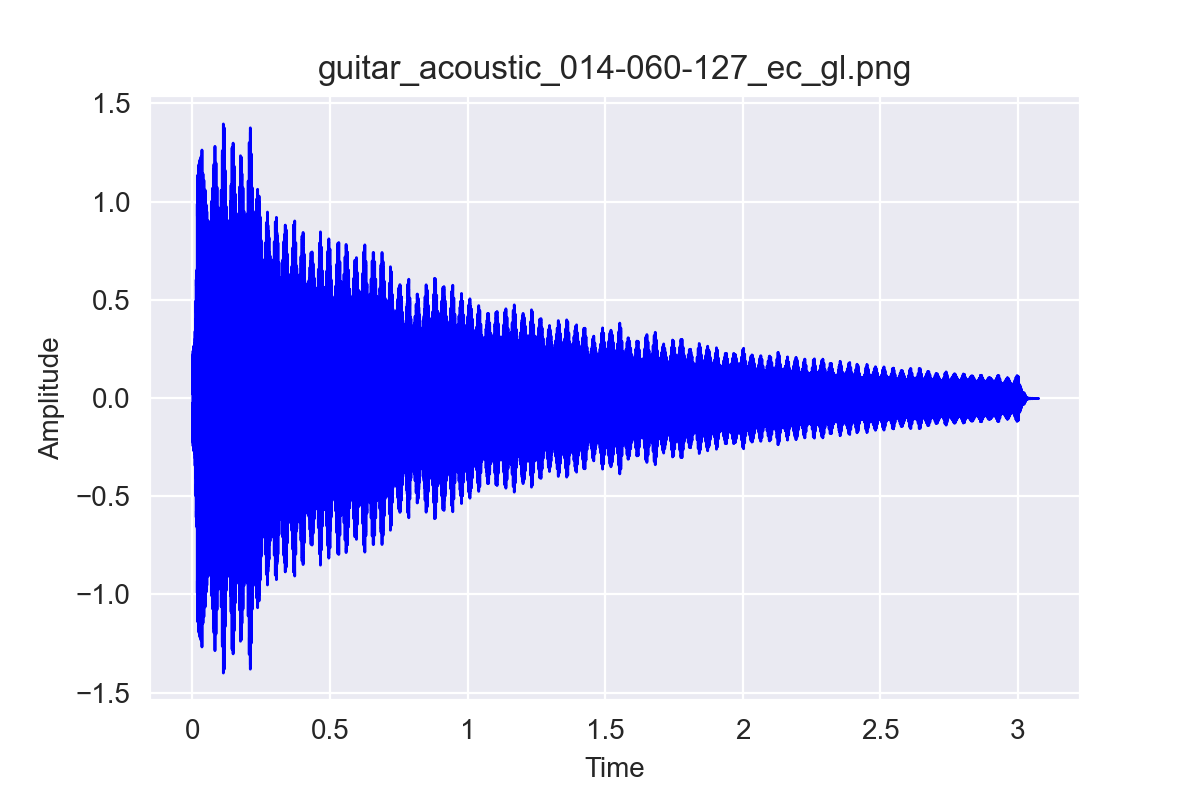
\includegraphics[width=0.50\textwidth]{images/appendix/mel_double_stride/guitar_acoustic_014-060-127_ec_gl.png}}\\
        without post-processing ~(a) & output with post-processing ~(b)
    \end{tabular}}
    \caption{Difference between acoustic guitar output signals without and with post-processing using 2D convolutional double-stride network and Griffin-Lim with log-mel spectrograms.}
    
\end{figure}

\begin{figure}[htb!]
    \centering
    \captionsetup{justification=centering}
    \makebox[\textwidth][c]{\begin{tabular}{@{}cc@{}}
        \makebox{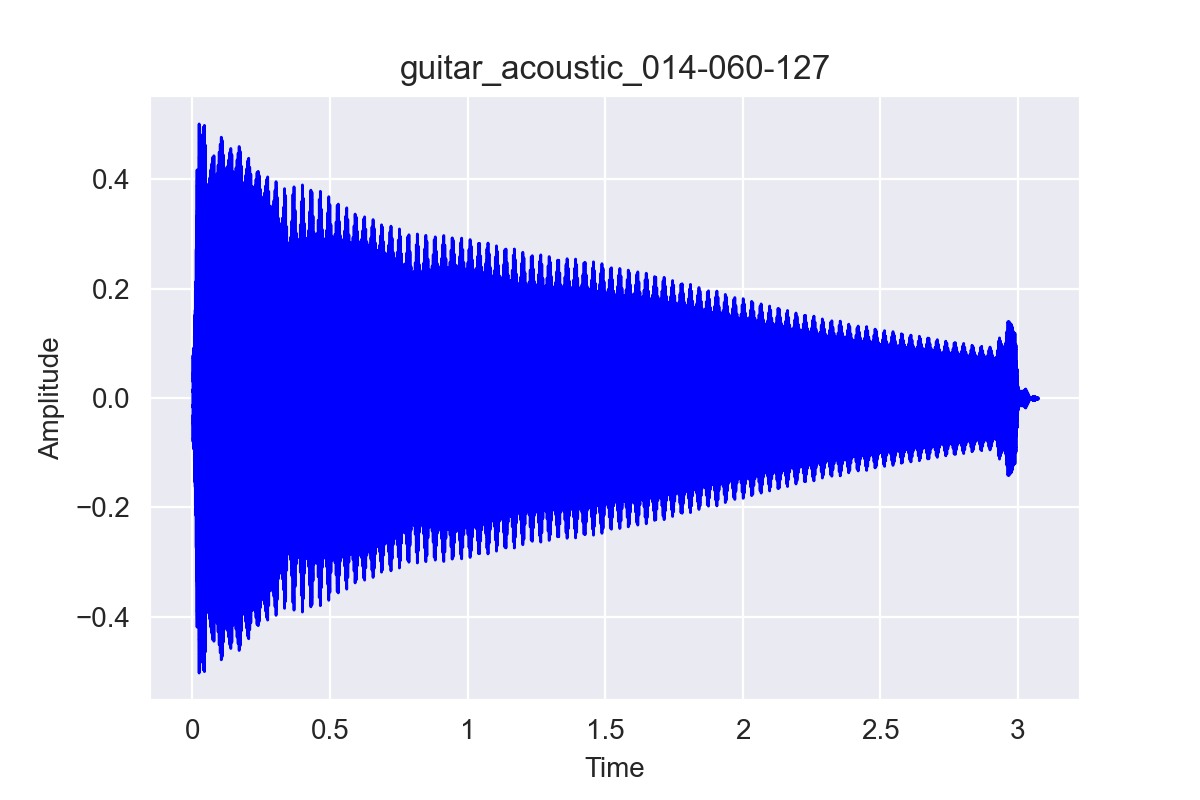
\includegraphics[width=0.50\textwidth]{images/appendix/mel_triple_stride/guitar_acoustic_014-060-127.png}}&
        \makebox{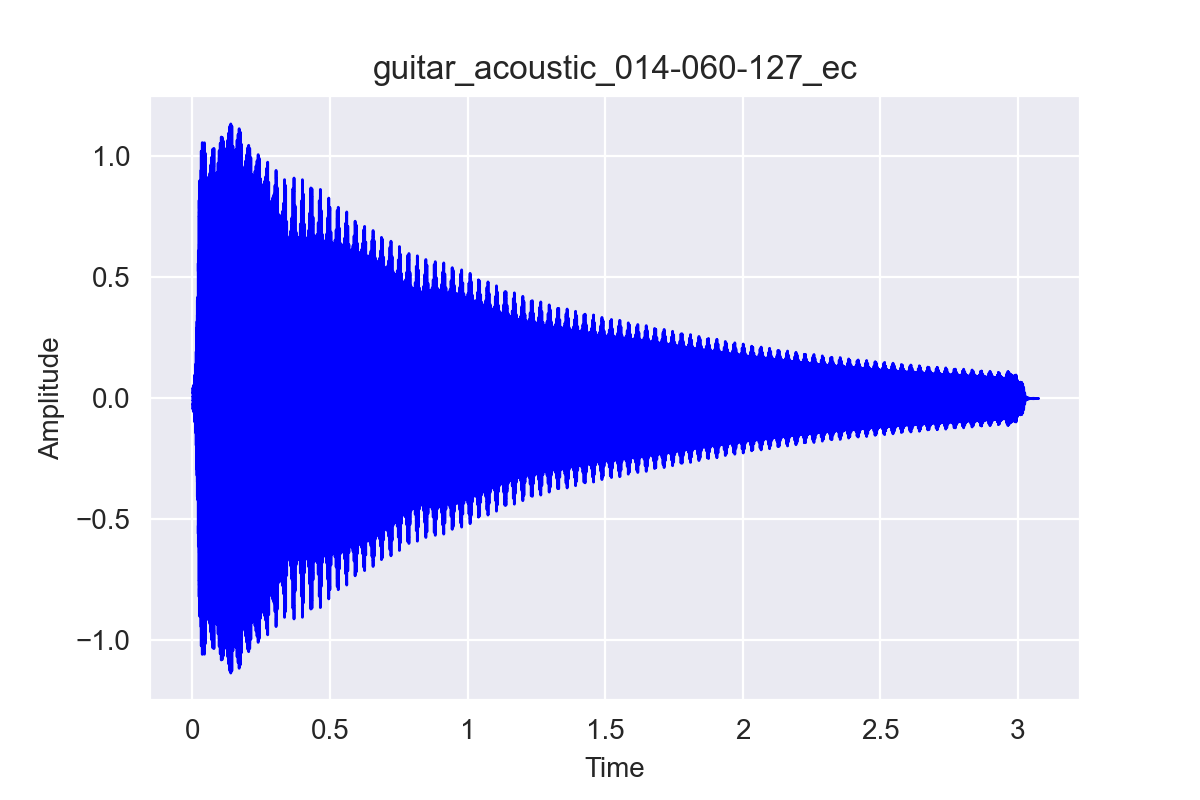
\includegraphics[width=0.50\textwidth]{images/appendix/mel_triple_stride/guitar_acoustic_014-060-127_ec.png}}\\
        without post-processing ~(a) & output with post-processing ~(b)
    \end{tabular}}
    \caption{Difference between acoustic guitar output signals without and with post-processing using 2D convolutional triple-stride network and original phase with log-mel spectrograms.}
    
\end{figure}

\begin{figure}[htb!]
    \centering
    \captionsetup{justification=centering}
    \makebox[\textwidth][c]{\begin{tabular}{@{}cc@{}}
        \makebox{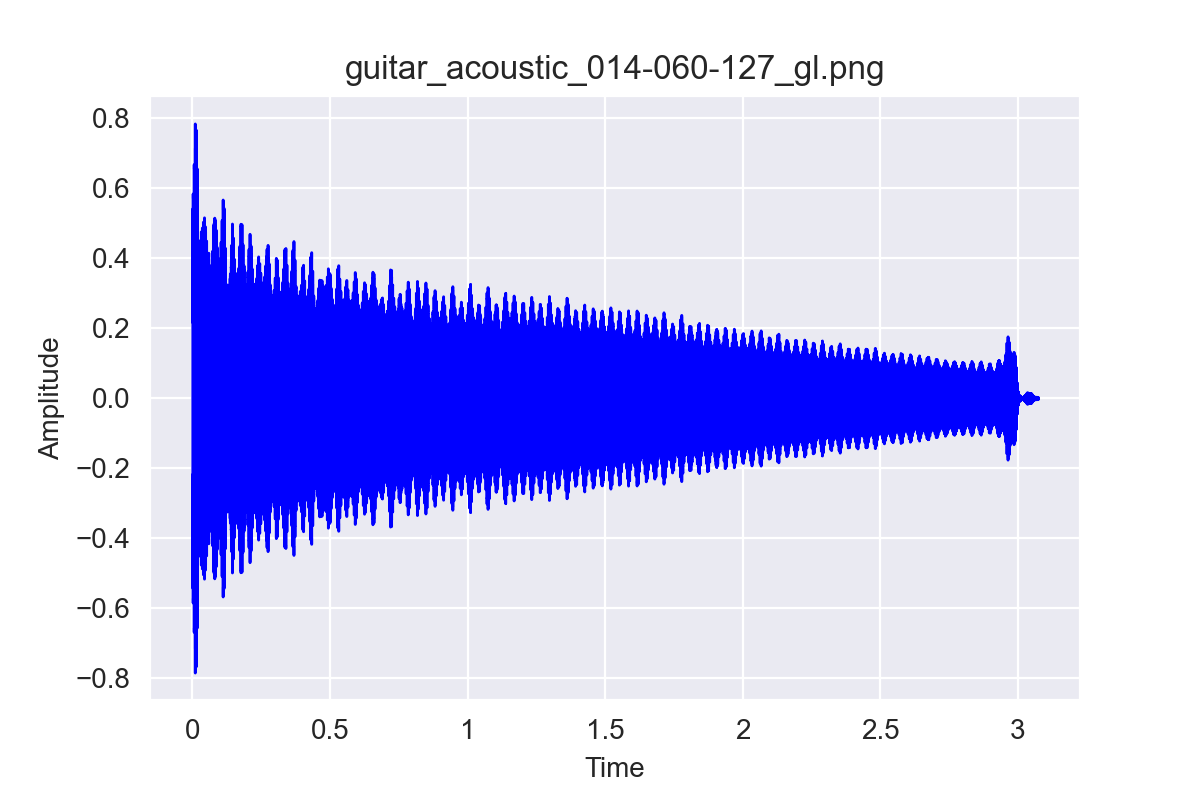
\includegraphics[width=0.50\textwidth]{images/appendix/mel_triple_stride/guitar_acoustic_014-060-127_gl.png}}&
        \makebox{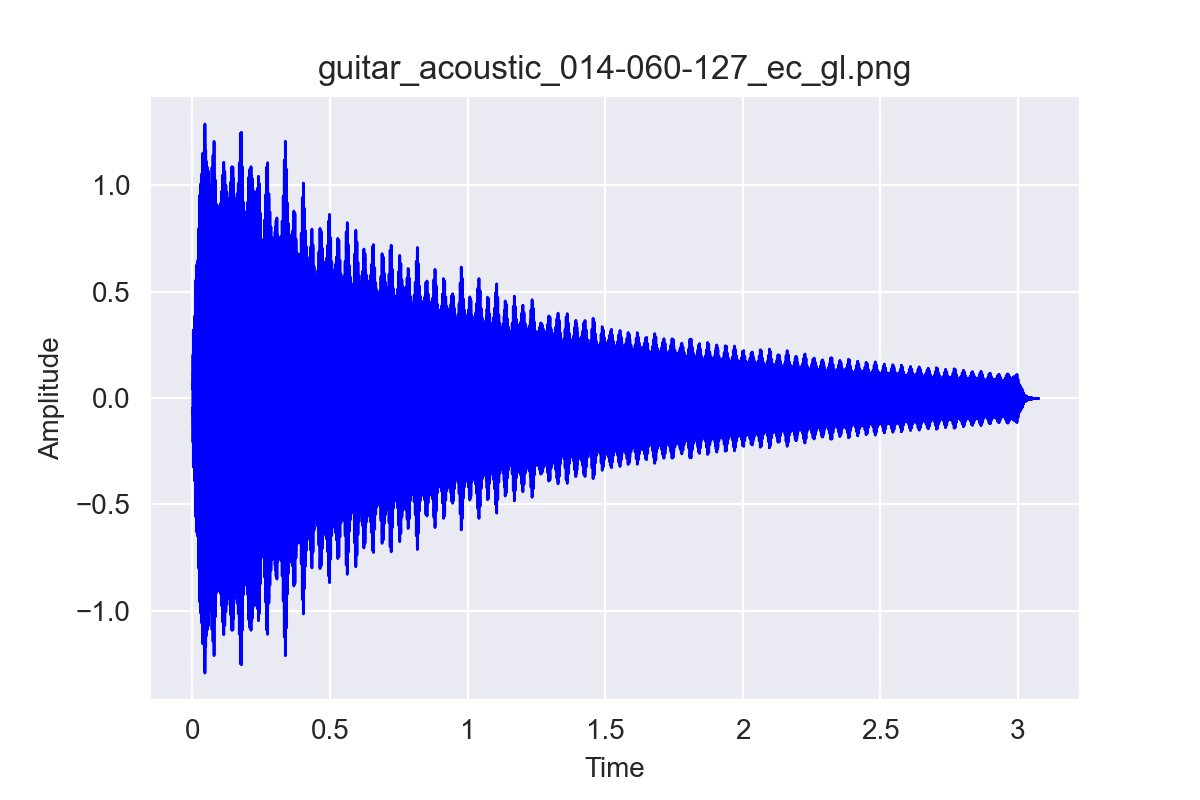
\includegraphics[width=0.50\textwidth]{images/appendix/mel_triple_stride/guitar_acoustic_014-060-127_ec_gl.png}}\\
        without post-processing ~(a) & with post-processing ~(b)
    \end{tabular}}
    \caption{Difference between acoustic guitar output signals without and with post-processing using 2D convolutional triple-stride network and Griffin-Lim with log-mel spectrograms.}
    
\end{figure}



\begin{figure}[htb!]
    \centering
    \captionsetup{justification=centering}
    \makebox[\textwidth][c]{\begin{tabular}{@{}cc@{}}
        \makebox{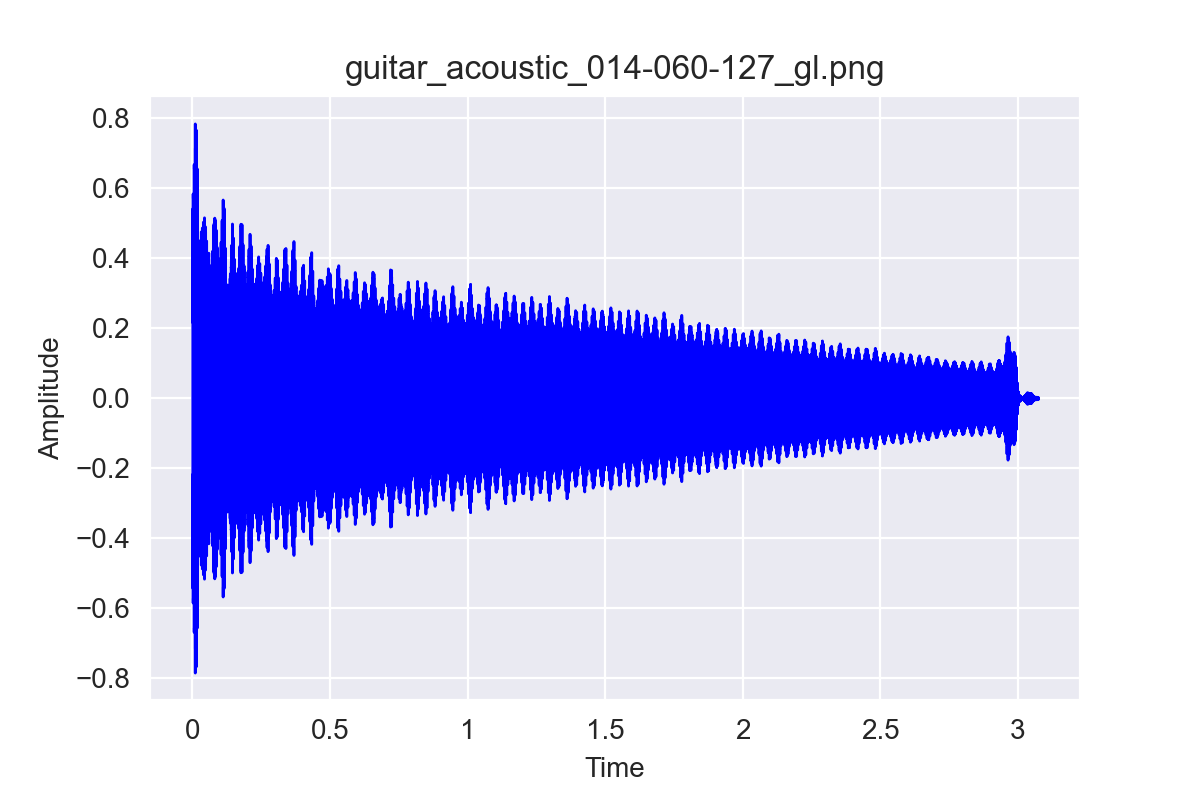
\includegraphics[width=0.50\textwidth]{images/appendix/mel_triple_stride/guitar_acoustic_014-060-127_gl.png}}&
        \makebox{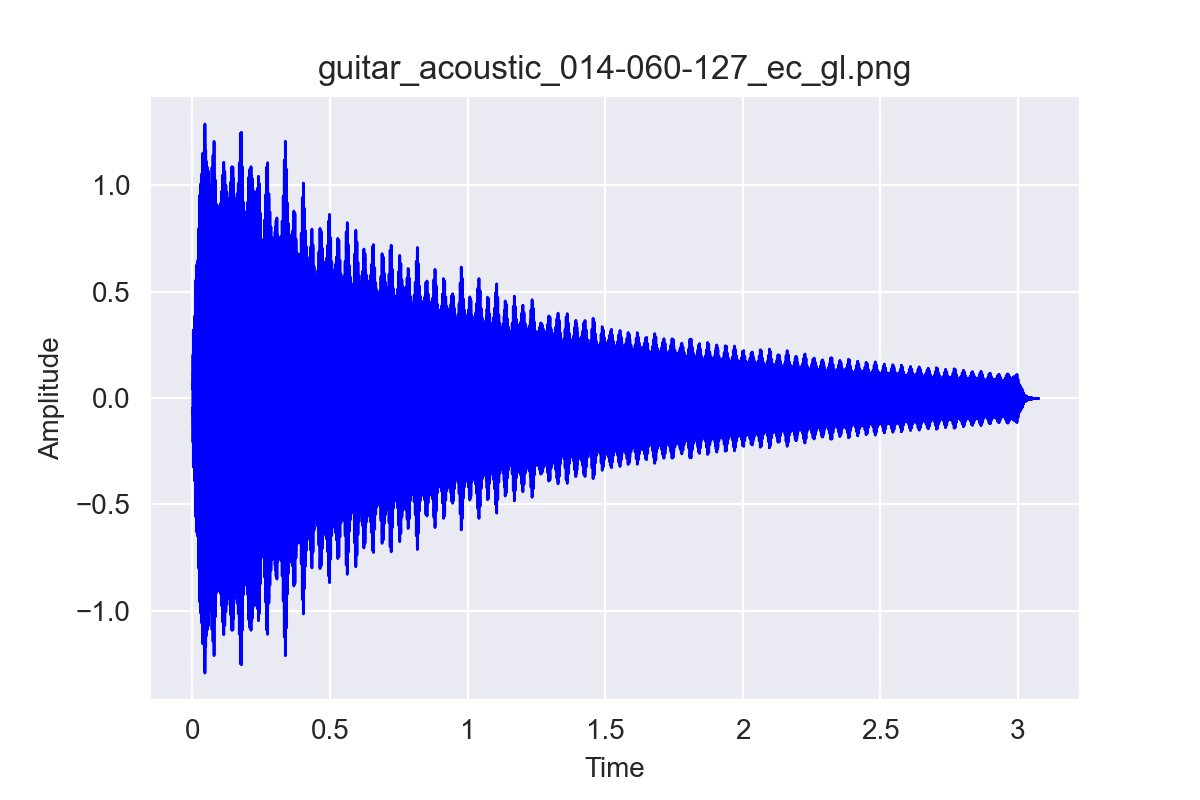
\includegraphics[width=0.50\textwidth]{images/appendix/mel_triple_stride/guitar_acoustic_014-060-127_ec_gl.png}}\\
        without post-processing ~(a) & with post-processing ~(b)
    \end{tabular}}
    \caption{Difference between acoustic guitar output signals without and with post-processing using 2D convolutional triple-stride network and Griffin-Lim with log-mel spectrograms.}
    
\end{figure}